\documentclass[11pt]{article}
\usepackage[margin=1in]{geometry}
\usepackage{amsmath,amssymb,booktabs,graphicx,hyperref}
\hypersetup{colorlinks=true,linkcolor=blue,citecolor=blue,urlcolor=blue}
\makeatletter\let\rowinput\@@input\makeatother
\newcommand{\D}{\Delta}
\title{Certifying best-of-$N$ verifier comparisons with fallible answer judgments}
\author{Yunjie Guo \qquad Hanqing Yang\\[2pt]
\small Independent Researcher, Suzhou, China\\
\small Correspondence: \texttt{hanqing.yang189@gmail.com}}
\date{}
\begin{document}
\maketitle
\begin{abstract}
A comparison between two mathematical verifiers can depend on a small number of uncertain answer grades. On a fixed generation pool, each answer contributes its grade times the difference in its probabilities of selection. We use this established linear comparison to ask how to spend a budget when preliminary judgments can be wrong. Given an upper bound on their error count, we derive the smallest attainable worst-case interval width both before provisional grades arrive and after they are available for selective adjudication. We replay 1,390,800 eligible responses from two public archives. On AceMath MATH-500 at eight draws, 437 reliable answer checks establish a 1.21 percentage-point lead, but 13 adverse grade changes can erase it. In the Lightman full-pool comparison, assuming at most five errors in either of two automatic grading rules gives intervals that exclude the archived 5.8-point gap. After calibrating the error bound by probability sampling, all six primary intervals contain zero. At the same adjudication budget, directly sampling signed grading errors gives narrower median intervals in all six settings. The minimax design is useful when an error ceiling can be defended and a guarantee across all compatible grades is required. Estimating a ceiling can be costly when the aim is a statistical comparison.

\end{abstract}

\section{Which grades can change the decision?}
A team replacing a verifier has a pool of mathematical solutions scored by both systems. In a best-of-$N$ trial each verifier chooses one solution from the same $N$ attempts. Getting the right answer earns one point. The comparison looks expensive to check if thousands of attempts exist per problem. Yet two solutions can carry the same final answer, and both verifiers may assign that answer nearly the same probability of winning. Even a difficult grading decision then has little effect on the comparison. Conversely, one mistaken judgment on a heavily favored answer can survive extensive review of other answers.

We ask two operational questions. How many answers must be checked before every admissible completion of the grades gives the same ordering? Once all answers have grades, how many adverse changes suffice to erase that ordering? These questions address a fixed benchmark and a specified inference budget. Publishing a point estimate alone answers neither. A standard error across questions describes another source of variation.

Our starting point is the classical idea of bounding differences between ranked systems with incomplete judgments \cite{carterette,tan}. We specialize it to the selection law of two mathematical verifiers, account exactly for ties and missing attempts, and pool repeated answer strings before prioritizing checks. We then allow errors in the judgments already returned. The main design result gives a sharp worst-case width for any combination of unreviewed, ordinarily reviewed and reliably adjudicated answers. It yields a closed-form ordering and a one-dimensional budget search. We test its practical implications by hiding and revealing archived final-answer grades. A second design uses provisional grades to decide which entries merit reliable adjudication. We challenge its error allowance using observed disagreements between two automatic answer rules and the published verdicts. Review prices are hypothetical.

\section{Estimand and winner probabilities}
For each of $Q$ equally weighted problems, fix $M$ generation slots, the returned answers, and two real-valued score vectors. Draw a size-$N$ subset of slots uniformly without replacement. Ignore ineligible attempts. If the subset has no eligible attempt, both systems receive zero. Each system selects a maximum-score eligible candidate, breaking ties uniformly. Both systems can be compared on the same draw even though their marginal winner distributions suffice for a difference in mean accuracy. This calculation does not identify how frequently they disagree on a particular draw.

Number eligible slots in descending score order starting at one. With distinct scores, the finite-pool order statistic used by Jacobson et al. \cite{jacobson} gives rank $r$ winner probability
\[
 p_r(N)=\binom{M-r}{N-1}\big/\binom{M}{N}.
\]
The other $N-1$ draws must come from lower ranks or missing slots. For a tie block occupying ranks $r$ through $s$, assign each member the average of $p_r,\ldots,p_s$. To see this, randomly permute that block before the draw. The first selected member in this permutation is uniformly distributed over the sampled members of the block. Thus scores may be discrete and even an all-tied block is admissible. A binomial coefficient is zero when its lower argument exceeds its upper argument.

Let an audit unit $i$ denote an exact answer within a problem, or a single response when rationale correctness is the target or answer grades cannot be shared. Write $a_i,b_i$ for the two winner probabilities summed over the unit's members and divided by $Q$. Let $d_i=a_i-b_i$ and $y_i\in\{0,1\}$ be the grade. The benchmark improvement is $\D=\sum_i d_i y_i$. Each problem has the same total eligible-winner mass under both systems, hence $\sum_i d_i=0$. Before any review the upper endpoint is half the $\ell_1$ distance between the two mass vectors. Pooling answer-equivalent candidates can only shrink this distance, by the triangle inequality. Oppositely signed candidate differences can cancel exactly inside one answer. All calculations in the released runner use integer binomial counts and a common multiple of tie sizes through the sign comparison.

\section{Partial review and erroneous judgments}
Partition the units into $G$ (reliably adjudicated), $R$ (ordinary reviews) and $U$ (unreviewed). Read $z_i$ on $G\cup R$, assume $y_i=z_i$ on $G$, and permit at most $e$ discrepancies on $R$. For an unreviewed unit any binary grade is possible. Write $S_k(V)$ for the sum of the $k$ largest elements of a nonnegative multiset, taking all elements if necessary. Let $T=\sum_{G\cup R} d_i z_i$ and $f_i=d_i(1-2z_i)$. The sharp endpoints are
\begin{align*}
 L &= T+\sum_{U}\min(0,d_i)-S_e(\{(-f_i)_+:i\in R\}),\\
 H &= T+\sum_{U}\max(0,d_i)+S_e(\{(f_i)_+:i\in R\}).
\end{align*}
Each endpoint is attained by independently setting the unknown grades and taking the most adverse permitted ordinary-label flips in its direction. The interval is the convex hull of feasible values. Some interior values can be unattainable. $L>0$ or $H<0$ certifies the sign even when the audit is stopped after inspecting the endpoints. No sampling model for correctness is required. The error allowance must cover actual errors for that interpretation.

For complete ordinary labels, orient $d$ toward the observed winner. Each label flip can reduce its margin by at most $[d_i(2z_i-1)]_+$. Sort the positive reductions. The shortest prefix whose sum reaches the margin is the exact minimum number of flips that erases a strict lead. A tie has radius zero. This sensitivity calculation locates how easily the result could change. It supplies no evidence that a published answer was graded incorrectly.

\subsection{Optimal allocation across review tiers}
Put $w_i=|d_i|$ and sort the weights $w_1\geq\cdots\geq w_m$. The worst-case width over all returned binary grades, for a fixed review design, is
\begin{equation}
 W(G,R,U)=\sum_{i\in U}w_i + S_{2e}(\{w_i:i\in R\}). \label{eq:width}
\end{equation}
Indeed, two truths compatible with a common transcript can disagree on at most $2e$ reviewed ordinary units. Conversely, split the largest $\min(2e,|R|)$ ordinary weights into two sets of at most $e$ each. On these units choose extreme grades to maximize the distance between truths. Set the transcript equal to the first truth on one set and to the second on the other. They agree on $G$ and may differ at every unreviewed unit. This attains (\ref{eq:width}). The two endpoints can involve different error locations.

\paragraph{Design theorem.}
Fix counts $g=|G|$ and $b=|R|$. An optimal fixed design sends the $g$ largest weights to reliable adjudication and the next $b$ to ordinary review. Its worst-case width, with $P_j=\sum_{i=1}^j w_i$, is
\begin{equation}
 P_m-P_{g+b}+P_{g+\min(b,2e)}-P_g. \label{eq:design}
\end{equation}
For a proof, exchange a smaller gold weight with a larger weight outside $G$. The affected term of (\ref{eq:width}) is coordinatewise nondecreasing, so moving the smaller weight outside cannot increase width. After arranging $G$, exchange a smaller ordinary weight $v$ with a larger unreviewed weight $u$. The tail sum on $U$ falls by $u-v$ and the top-$2e$ sum increases by at most $u-v$. Repeating these exchanges gives (\ref{eq:design}). When ordinary review costs one credit, gold costs an integer $c$, and $B$ credits are available, enumerate $0\leq g\leq\min(m,\lfloor B/c\rfloor)$ and set $b=\min(m-g,B-cg)$. A prefix sum evaluates each allocation in constant time after sorting. This solves a nonadaptive, worst-transcript width objective. It permits ties between optimal allocations and gives no promise of the shortest realized sign audit.

Two boundaries clarify the role of review reliability. If $b\leq2e$, ordinary review cannot shrink the worst-case width at all. With $g=0$, $e=0$, the rule reduces to sorting by absolute mass difference. For an example where both tiers help, let the absolute weights be $(15,5,5,4,4,3,2,2)$. Give the first two positive signs and all others negative signs, and divide by 20 to obtain a difference of probability vectors. In unnormalized units, with $B=7$, $c=3$ and $e=1$, seven ordinary reviews leave a worst-case width of $22$. Two gold reviews with one remaining ordinary review leave $20$. One gold and four ordinary reviews reduce the width to $17$.

\subsection{Choosing which provisional judgments to adjudicate}
Consider a different point in an audit. The ordinary reports on $R$ have arrived. A reviewer can now afford $h$ reliable checks of distinct entries in $R$. Keep the rest of the benchmark fixed. The allowance $e$ refers to the original $R$, hence finding $k$ discrepancies leaves at most $e-k$ errors. This distinction matters when an existing automatic grader can supply provisional reports before expensive verification.

\paragraph{Conditional design theorem.}
Classify entries by the sign of $f_i=d_i(1-2z_i)$ and sort their absolute weights in decreasing order within each class. Zero effects can be placed in either class. For class $j$ let $T_j(t,e)$ be the sum of the next $e$ weights after its first $t$, counting all available weights if fewer remain. The smallest worst-branch width after $h$ upgrades, including over sequential deterministic choices of the entries, is
\[
 \sum_{i\in U}|d_i|+\min_{t}\left[T_-(t,e)+T_+(h-t,e)\right],
\]
where both allocations must fit their class sizes. Upgrade the respective prefixes. Sorting takes $O(|R|\log |R|)$ and the split search takes $O(h)$ with prefix sums.

For any deterministic strategy, follow the branch on which every reliable check confirms its provisional grade. This branch is feasible even at $e=0$. Its unresolved width is the sum of the largest $e$ remaining positive effects and the largest $e$ remaining negative magnitudes, plus the fixed unknown width. For each split, removing the largest weights on each side minimizes both terms by exchange. This lower-bounds every strategy. Select the minimizing split in advance. A branch with $k$ discrepancies has the same remaining lists and a smaller or equal allowance $e-k$. Its width cannot exceed the all-confirming branch's width, which proves attainment. The objective concerns width conditional on the provisional transcript. A strategy optimized for the probability of an early sign decision has a different objective.

For example, take provisional correction effects $(-8,10,10)$ in common weight units with $e=h=1$. Checking either size-ten entry leaves worst-case width $18$ on this group. Checking the size-eight entry leaves width $10$ because every remaining correction has the same direction.

\paragraph{An allowance with measured risk.}
Draw $s$ units uniformly without replacement from a score-selected $R$ of size $m$, adjudicate them, and count $k$ discrepancies. For $H_K\sim\mathrm{Hypergeom}(m,K,s)$ let $K^+=\max\{K:\Pr(H_K\leq k)>\alpha\}$ over feasible totals. The lower-tail test has size at most $\alpha$ by discreteness. Its inversion upper-bounds the total discrepancy count with probability at least $1-\alpha$. Remove the sampled entries and use $e=K^+-k$ on the remainder. On that single coverage event all subsequent deterministic intervals contain the stipulated target. If later checks exhaust the allowance and reveal another discrepancy, the compatible set is empty and the audit must report that outcome. This construction requires a reliable comparison grade on sampled units and an actual probability sample. Only this calibration step carries sampling risk. The finite-population inversion itself is standard.


\section{Evidence and comparisons}
\paragraph{Archives.}
The OpenAI scored evaluation pool \cite{lightman} supplies a process-supervised reward model (A) and an outcome-supervised model (B) on the same generations. We follow the original evaluator's attempt denominator of 1,860 and exclude null answers from selection. The second release, AceMath-RewardBench \cite{ace}, supplies paired 72B (A) and 7B (B) reward scores on 64 solutions per problem, eight from each of eight generators. We join the two files by problem index within each subject and require identical ordered answer and grade vectors. The original AceMath evaluator uses 100 random ordered subsets and selects the first maximum, which implements uniform tie breaking in expectation. At $N=8$ our exact subject accuracies for the two models are all within 0.10 percentage points of the corresponding published cells. The seven subjects are analyzed separately. MATH-500 is shared in subject matter and benchmark identity across the two releases. The releases provide different generations and reward models.

\paragraph{Replay.}
We specified $N=8,32,M$ before computing outcomes. Both graders see the same eligible pool. We use the archived binary answer grade throughout. The primary unit combines equal nonempty extracted strings within a problem. Empty or unavailable strings among eligible responses receive separate units. We count mixed-grade groups. Where a mixed group exists, the first-occurrence grade defines a string-level sensitivity analysis and response-level results identify the original graded contrast. No algebraic simplification is applied. We retain all problems, including those with no leverage for a particular budget.

We hide the labels for the purposes of selecting a review order and reveal them to evaluate the stopping rule. The proposed order sorts by $|a_i-b_i|$. A pooled baseline sorts by $\max(a_i,b_i)$, so it reviews likely winners from either verifier. Both use stable input order for priority ties. We also compute the expected interval width for a uniform random permutation at a fixed budget: after $b$ of $m$ units it equals $(1-b/m)\sum_i |d_i|$. All review counts include only grades revealed, assuming unit cost for each exact answer or response. They describe an archive replay. The grader was not rerun and no human time was measured. As a design sensitivity we give reliable adjudication a price of two or five ordinary judgments and allow up to five errors among ordinary judgments.

The study protocol records the initial design, the two-tier cost sensitivity specified before examining outcomes, and two follow-ups prompted by the first replay. The latter address tie priorities and whole-question review costs. Exhaustive tests enumerate candidate subsets, admissible grades, corruptions and small review allocations. The replication package contains all budget rows, including inconclusive error-tolerant comparisons.

\paragraph{Reviewing an answer once.}
At $N=8$, on MATH-500, the two AceMath reward models score 86.69\% and 85.48\% in expectation over subsets. The archive contains 32,000 eligible responses and 7,978 question--answer units. With error-free reveals, the contrast order certifies the 1.21-point advantage after 437 answer judgments. The same priority applied to response-specific grades takes 11,942 judgments. Grouping by answer still helps without changing the priority to the contrast: pooling likely winners from the two systems requires 870 answer judgments (Table~\ref{tab:eight}). The two efficiencies arise from different operations, sharing grades between responses and canceling the probability that both systems assign to an answer.

\begin{table}[htbp]\centering\small
\caption{Audits at $N=8$. Gap is A minus B in percentage points. Checks count reveals until the sign is certified with $e=0$. Response and answer use absolute mass difference. Pool uses the larger winner mass on answer units. Radius is the smallest number of complete answer grades that could erase the lead.}\label{tab:eight}
\begin{tabular}{lrrrrrrr}\toprule
 & & & & \multicolumn{3}{c}{Checks to certify sign} & \\
Collection & Tasks & Answers & Gap & Response & Pool & Answer & Radius\\\midrule
\rowinput at_eight.tex
\bottomrule\end{tabular}
\end{table}

The initial MATH-500 answer-level gap width is 11.28 points. After reviewing 797 answers it is 0.78 points under contrast priority, 2.76 under pooled priority and 10.15 in expectation under uniform ordering. Allowing five errors in these 797 reviews still puts the gap between 0.21 and 2.10 points. In contrast, after revealing every Gaokao answer, even the sign at $N=8$ cannot be certified if five reviews might be wrong. Its complete-label radius is four. MMLU STEM requires 250 adverse changes at the same budget. These are sensitivity thresholds for mathematical answer grades.

\begin{figure}[htbp]\centering
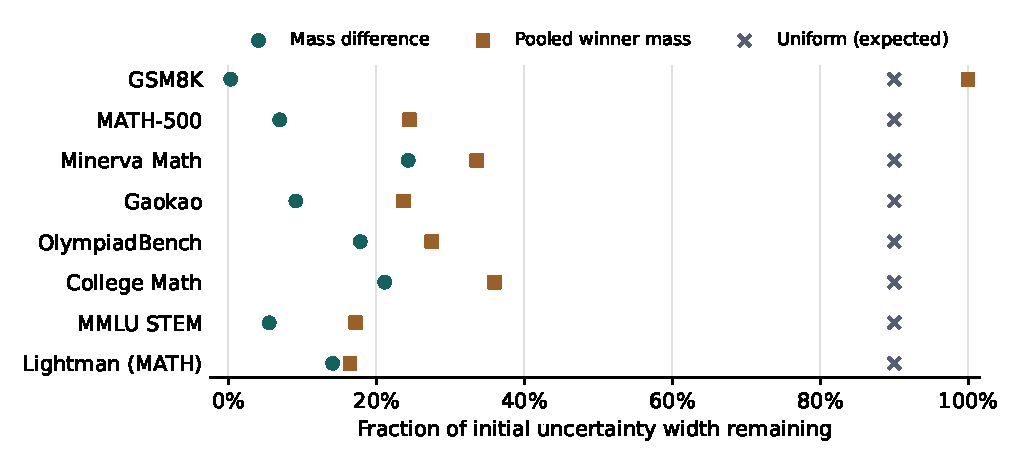
\includegraphics[width=.94\linewidth]{widths.pdf}
\caption{Residual answer-level uncertainty after reviewing $\lfloor 0.1m\rfloor$ of $m$ answers at $N=8$ with $e=0$. Each row is normalized by its own initial width. Uniform uses the exact expected width.}\label{fig:width}
\end{figure}

\paragraph{A second verifier family at a larger search depth.}
The Lightman release supplies 815,632 eligible scored responses for 500 problems, out of 930,000 generation slots. At $N=1{,}860$ we recover the published 78.2\% process-verifier and 72.4\% outcome-verifier accuracies. The target can be certified after 245 answer-unit checks under the first-occurrence grading convention. At $N=8$, it takes 20,356 such checks for a 0.69-point lead, and six adverse grade changes can erase it. At the full pool the lead rises to 5.80 points and the radius rises to 29. Thus the fall in Minerva's radius with increasing $N$ is not universal.

All 8,987 AceMath problem pools had consistent published grades within the declared answer units. There was one mixed-grade group among 94,816 Lightman units. It contained 67 responses. Choosing either shared binary grade can move the gap by at most 0.0014 points at $N=8$, 0.0015 at $N=32$ and 0.20 at $N=1{,}860$. The aggregate response-level gains using the original grades are 0.693, 2.078 and 5.800 points respectively. The answer-level checks for this release are conditional on the chosen resolution. Pooling without inspecting that assumption would conceal the inconsistency.

\paragraph{Generation budget and review reliability.}
On Gaokao the fully graded uniform-tie comparison changes from $+0.78$ points at $N=8$ to $-0.32$ at $N=32$ and $-1.04$ at $N=64$. Two adverse answer-grade changes suffice to erase the middle comparison. On Minerva Math the advantage grows from 3.13 to 4.78 points between $N=8$ and 64, while its radius falls from 23 to 13. Higher confidence in the ordering under missing labels can coexist with greater sensitivity to individual grades: a maximum over more draws can concentrate selection mass on fewer answers.

\begin{table}[htbp]\centering\scriptsize
\caption{Effect of generation budget on each fixed pool. Columns within each block use $N=8,32,M$. $M=64$ in AceMath and 1,860 in Lightman. Counts use exact answers and contrast priority.}\label{tab:scaling}
\begin{tabular}{lrrr rrr rrr}\toprule
&\multicolumn{3}{c}{Gap (points)}&\multicolumn{3}{c}{Checks to certify}&\multicolumn{3}{c}{Erasure radius}\\
Collection & 8 & 32 & Full & 8 & 32 & Full & 8 & 32 & Full\\\midrule
\rowinput scaling.tex
\bottomrule\end{tabular}
\end{table}

\paragraph{When adjudication is worth its cost.}
At $N=8$ on MATH-500, give an auditor 797 credits, set $e=5$, and charge five credits for reliable adjudication. Spending all credits on ordinary review gives a worst-transcript gap width of 1.96 points. Spending them exclusively on adjudication gives 5.30 points. The minimax design uses 23 reliable and 682 ordinary checks for a worst-case width of 1.52 points. At a smaller budget of 79 credits, the minimizer uses ordinary review alone. On GSM8K at $N=8$ with a 10\% budget and the same costs, the corresponding mixed width is 0.17 points against 0.52 and 0.51 points for the single-tier options. The economic premise is illustrative. The archive permits computation of the design for other costs before a reviewer is assigned.


\paragraph{Sensitivity to tie priority.}
The Gaokao reversal prompted a follow-up check on every subject. Within each tied score block, placing correct candidates first gives that verifier its best feasible value, and putting them last gives its worst. Subtract opposite extremes for the two verifiers to bound the gap over independently chosen tie priorities. This uses complete labels only to measure sensitivity. For Gaokao the interval is $[+0.73,+0.83]$ points at $N=8$, $[-0.45,-0.19]$ at 32 and $[-1.30,-0.78]$ at 64. Every such policy preserves the reversal on these fixed grades. The four-label erasure radius at 64 addresses a different perturbation, namely changing grades under the declared uniform-tie policy.

\paragraph{If solving one problem settles several answers.}
As a second follow-up, charge one check for adjudicating all answer units of a question. Its interval then collapses by $\sum_{i\in q}|d_i|$, so review questions in descending order of that sum. For complete grades, allow arbitrary changes within an affected question. The greatest loss for that question is its observed, winner-oriented contribution minus its lowest feasible contribution. Sorting these losses gives the minimum number of affected questions needed to erase the lead. At $N=8$ on AceMath MATH-500, 79 complete question checks certify the sign and adverse changes concentrated in six questions can erase it. On Gaokao the counts are 112 and two. At $N=32$ on Gaokao, changes within one question suffice. The calculation allows multiple changed judgments per problem. It does not assume that all those changes follow from substituting one valid answer key.

\subsection{How often does the mixed design help?}
The initial sensitivity grid contains 96 cells: eight collections, three generation budgets, two review budgets and two gold prices. Each cell compares the minimax width to the better of ordinary-only and gold-only review, with $e=5$. At the 1\% review budget, the combined design reduces width in 7 of 24 cells at price two and 2 of 24 at price five. At 10\% the counts are 15 and 14 respectively (differences above $10^{-10}$ percentage points). Across the 24 cells at the 10\% budget the median reductions are 0.037 and 0.013 points. These are factorial design cells on fixed archives, not independent model comparisons. The mixed design can help materially in individual settings, while most settings yield a small absolute improvement or a tie.

\subsection{When the error allowance must be estimated}\label{sec:calibration}
We use Lightman's original reference-answer strings to produce a provisional verdict for each answer unit. Literal matching accepts a nonempty exact match after stripping surrounding whitespace. A second rule also accepts exact rational equality for supported integer, decimal and simple fraction forms. Both ignore the published verdict when grading. The reliable return in this retrospective test is the archived first-occurrence verdict. Agreement measures fidelity to this declared target. It gives no estimate of human annotator accuracy. These simple rules permit a reproducible challenge to the small-error assumption on a corpus with released references.

At each $N$, take the first 10\% of answer units by $|d_i|$ and discard zero-weight units from this prefix. Other nonzero units stay unreviewed. On this provisional set, the literal and rational rules exceed five discrepancies at every budget (Table~\ref{tab:proxies}). At $N=1{,}860$ a literal-grader interval computed with $e=5$ is $[2.0,4.0]$ points and the rational version gives $[3.0,5.0]$. Both exclude the archived gap of $5.8$ points despite retaining its sign. The original sensitivity examples at $e=5$ therefore cannot be interpreted as measured guarantees for either grading rule.

We next calibrate as above, taking $s=\min(256,\lfloor |R|/4\rfloor)$ and $h=\min(128,\lfloor(|R|-s)/4\rfloor)$. Both graders share the same calibration sample within each $N$. Each cell uses $\alpha=1/120$, giving simultaneous coverage of at least 95\% across the six cells by the union bound. We compare adjudication of the largest remaining $|d_i|$ against the conditional design with identical $s,h$. At the two smaller generation budgets the two choices have equal worst-branch widths in the prespecified seed. At full depth the conditional split reduces that width from 20.0 to 17.4 points for literal matching and from 16.4 to 15.0 for rational matching. Every primary calibrated interval contains zero, including the rational full-depth interval whose lower endpoint is exactly zero.
\begin{table}[htbp]\centering\small
\caption{Observed disagreement and calibrated conditional-upgrade intervals. $k/s$ counts sampled disagreements, $e$ is the calibrated upper bound on remaining errors before upgrades, and $h$ counts subsequent checks. Endpoints are percentage points for the archived gap.}\label{tab:proxies}
\begin{tabular}{rlrrrrr}\toprule
$N$ & Grader & Disagree / $|R|$ & $k/s$ & $e$ & $h$ & Final interval\\\midrule
8 & Literal & 273/9,481 & 11/256 & 775 & 128 & $[-7.28,8.89]$\\
8 & Rational & 234/9,481 & 10/256 & 727 & 128 & $[-7.18,8.78]$\\
32 & Literal & 285/9,481 & 5/256 & 478 & 128 & $[-6.70,9.85]$\\
32 & Rational & 241/9,481 & 5/256 & 478 & 128 & $[-6.72,9.86]$\\
1,860 & Literal & 34/290 & 7/72 & 50 & 54 & $[-1.20,13.80]$\\
1,860 & Rational & 25/290 & 5/72 & 41 & 54 & $[0.00,12.80]$\\
\bottomrule\end{tabular}
\end{table}

\paragraph{Comparison with direct probability sampling.}
After seeing the primary results we added a comparator motivated by importance sampling for ranking comparisons \cite{schnabel}. It starts with the same provisional grades and leaves the same answers outside $R$ unknown. Split $R$ by the sign of $f_i$ and let $W_j$ be the total absolute weight in stratum $j$. Allocate $s+h$ draws in proportion to $W_j$, rounding to integer counts and ensuring at least one per nonempty stratum. Within each stratum sample independently with replacement with probabilities $|d_i|/W_j$. On each draw the disagreement indicator has mean equal to the unknown fraction of stratum weight that requires correction. Thus a binomial interval for each fraction, scaled by $W_j$ and signed, gives an interval for the correction to the provisional comparison. Add the sharp unknown endpoints outside $R$. We invert the two binomial tails per stratum, each at risk $1/480$, rounding endpoints outwards to a grid of $1/65536$. The resulting six-cell family has at least 95\% simultaneous coverage over random draws in each repetition. Repeated draws may reuse a grade. In the primary seed this used 322--330 distinct answers at the two smaller budgets (384 draws) and 108--109 at full depth (126 draws).

\begin{table}[htbp]\centering\small
\caption{Thirty-two sampling seeds on the same Lightman pool. Widths are medians in percentage points. Sign decisions count intervals strictly excluding zero. Each design uses the same upper limit on reliable checks.}\label{tab:control}
\begin{tabular}{rlrrrr}\toprule
& & \multicolumn{2}{c}{Median width} & \multicolumn{2}{c}{Sign decisions / 32}\\
$N$ & Provisional rule & Upgrades & Sampling & Upgrades & Sampling\\\midrule
8 & Literal   & 15.60 & 7.43 & 0 & 0\\
8 & Rational  & 15.29 & 7.22 & 0 & 0\\
32 & Literal  & 17.59 & 5.61 & 0 & 1\\
32 & Rational & 16.74 & 5.41 & 0 & 3\\
1,860 & Literal & 17.70 & 13.94 & 2 & 3\\
1,860 & Rational & 14.40 & 12.05 & 5 & 12\\
\bottomrule\end{tabular}
\end{table}
Direct sampling has the smaller median width in every cell (Table~\ref{tab:control}). At full depth with rational grading it certifies the sign in 12 of 32 replays, compared with five for calibrated upgrades and one for magnitude-only upgrades. These repetitions vary which units are checked on one archive. They describe sampling variability and supply no additional independent model pairs. A defensible externally specified error ceiling permits a deterministic audit. When the ceiling itself must be estimated, direct sampling can spend the same checks on estimating the weighted correction, a substantial advantage in this replay.

\section{Relation to prior work}
Carterette, Allan and Sitaraman \cite{carterette} choose relevance judgments to compare retrieval systems. Tan and Clarke's maximized effectiveness difference \cite{tan} bounds ranking differences over unknown judgments. For a linear effectiveness metric their shared-item variables give exactly our error-free endpoints: identify one relevance variable with a question--answer grade and its two rank weights with $a_i,b_i$. Selecting the largest $|d_i|$ then follows by subtracting the width after a single reveal. Moffat, Webber and Zobel \cite{moffat} already use targeted static and dynamic judgments for rank-weighted system comparisons. Schnabel et al. \cite{schnabel} use differences in systems' exposure probabilities in a variance-optimal importance sampler. Shared-answer cancellation, the rank kernel and clean-label priority therefore have direct antecedents. The direct-sampling comparator also uses the prediction-plus-estimated-correction principle of prediction-powered inference \cite{ppi}. Here the signed correction is estimated on one finite archive. Active comparison \cite{sawade} and active testing \cite{kossen} optimize statistical precision under limited labeling. Test-label corrections have changed model rankings on public benchmarks \cite{northcutt}. Our erasure radius holds model scores fixed and asks how few adverse corrections could suffice. Risk-limiting audits \cite{stark} can use random samples and a chosen risk limit to certify a decision. Our review counts impose a deterministic requirement over compatible truths. Section~\ref{sec:calibration} uses a common nominal risk to compare two sampling-based designs when the error ceiling is unknown.

Lightman et al. \cite{lightman} and Liu et al. \cite{ace} evaluate mathematical reward models through repeated subset draws. We study the effort and fragility of verifying their fixed-pool comparisons. Schweisthal et al. \cite{bon} use score ranks to estimate policy values for future samples via off-policy evaluation. Shah and Li \cite{hold} analyze the effects of repeated noisy scores and holdout evaluation. Here both score vectors are observed and fixed. Uncertainty enters through missing or potentially erroneous external grades. The largest-$e$ adjustment for a single endpoint also has the integer budgeted-uncertainty form of Bertsimas and Sim \cite{bertsimas}. Our narrower result couples the two endpoints through one fallible transcript: the sharp $2e$ width, the two-price allocation before grades arrive, and the optimal split between correction directions once they arrive. The empirical question is how much those choices change an audit on released verifier scores.

\section{Scope and implications}
A certificate attaches to the declared distribution over subsets, the tie policy, the fixed scores and the grading unit. It does not bound future prompt or generator shift. A solution can contain a faulty derivation and a correct final answer. Reviewing the process requires response-specific or step-specific judgments. Distinct strings can be mathematically equivalent, and unsupported canonicalization could merge inequivalent answers. Separate groups for distinct strings preserve more uncertainty. The sharpness statements range over independent binary assignments to the declared units. A known single correct option or known equivalences between strings would restrict that set. An adverse assignment need not correspond to changing a single mathematically consistent reference key. Errors may cluster by question or grader, and one incorrect reference can affect several units. The radius counts affected units, without assigning a probability or a cause. Reliable adjudication and constant costs are design assumptions that require evidence in a live deployment. Repeated checks by correlated judges need not yield a reliable tier.

The practical output is an audit target with a stated unit and budget. A reviewer can report the observed improvement, the interval for unrevealed answers, and the fewest grade changes sufficient to erase the lead. These quantities answer different questions even when they come from the same released rankings.
\paragraph{Data and software.} The repository includes the protocol, input hashes, exact evaluator, exhaustive checks, and per-problem results. The cited authors host the source data. \url{https://github.com/fightforbelief/p9-verifier-audit}
\paragraph{Declarations.} The authors declare no competing interests and no specific funding for this work.
\begin{thebibliography}{10}
\bibitem{carterette} B. Carterette, J. Allan and R. Sitaraman. Minimal test collections for retrieval evaluation. SIGIR, 2006. \url{https://ciir.cs.umass.edu/pubfiles/ir-475.pdf}
\bibitem{tan} L. Tan and C. L. A. Clarke. A family of rank similarity measures based on maximized effectiveness difference. IEEE TKDE, 2015. \url{https://arxiv.org/abs/1408.3587}
\bibitem{sawade} C. Sawade, N. Landwehr and T. Scheffer. Active comparison of prediction models. NeurIPS, 2012. \url{https://proceedings.neurips.cc/paper_files/paper/2012/file/92fb0c6d1758261f10d052e6e2c1123c-Paper.pdf}
\bibitem{northcutt} C. G. Northcutt, A. Athalye and J. Mueller. Pervasive label errors in test sets destabilize machine learning benchmarks. NeurIPS Datasets and Benchmarks, 2021. \url{https://arxiv.org/abs/2103.14749}
\bibitem{moffat} A. Moffat, W. Webber and J. Zobel. Strategic system comparisons via targeted relevance judgments. SIGIR, 2007. \url{https://doi.org/10.1145/1277741.1277806}
\bibitem{schnabel} T. Schnabel, A. Swaminathan, P. I. Frazier and T. Joachims. Unbiased comparative evaluation of ranking functions. ICTIR, 2016. \url{https://www.cs.cornell.edu/~adith/docs/UBCompEval.pdf}
\bibitem{bertsimas} D. Bertsimas and M. Sim. The price of robustness. Operations Research, 52(1), 35--53, 2004. \url{https://doi.org/10.1287/opre.1030.0065}
\bibitem{jacobson} A. Jacobson, Q. Xie and P. I. Frazier. Latency-aware adaptive Best-of-$N$. Appendix on finite-pool selection, 2026. \url{https://arxiv.org/abs/2611.07453}
\bibitem{ppi} A. N. Angelopoulos, S. Bates, C. Fannjiang, M. I. Jordan and T. Zrnic. Prediction-powered inference. Science, 382, 669--674, 2023. \url{https://arxiv.org/abs/2301.09633}
\bibitem{kossen} J. Kossen et al. Active testing: Sample-efficient model evaluation. ICML, 2021. \url{https://proceedings.mlr.press/v139/kossen21a.html}
\bibitem{stark} P. B. Stark. Sets of half-average nulls generate risk-limiting audits: SHANGRLA. Financial Cryptography and Data Security, 2020. \url{https://arxiv.org/abs/1911.10035}
\bibitem{lightman} H. Lightman et al. Let's verify step by step. ICLR, 2024. \url{https://arxiv.org/abs/2305.20050}
\bibitem{ace} Z. Liu et al. AceMath: Advancing frontier math reasoning with post-training and reward modeling. 2024. \url{https://arxiv.org/abs/2412.15084}
\bibitem{bon} J. Schweisthal et al. Efficient Best-of-N policy evaluation for inference-time alignment. 2026. \url{https://arxiv.org/abs/2610.09250}
\bibitem{hold} S. Shah and Y. Li. Holdout Best-of-N: Unbiased evaluation and its cost. 2026. \url{https://arxiv.org/abs/2610.08719}
\end{thebibliography}
\end{document}
